% Editable source for probe_profile.pdf, written by make_figures.py from analysis/profile_local.json
\documentclass[border=6pt]{standalone}
\usepackage{tikz}
\begin{document}
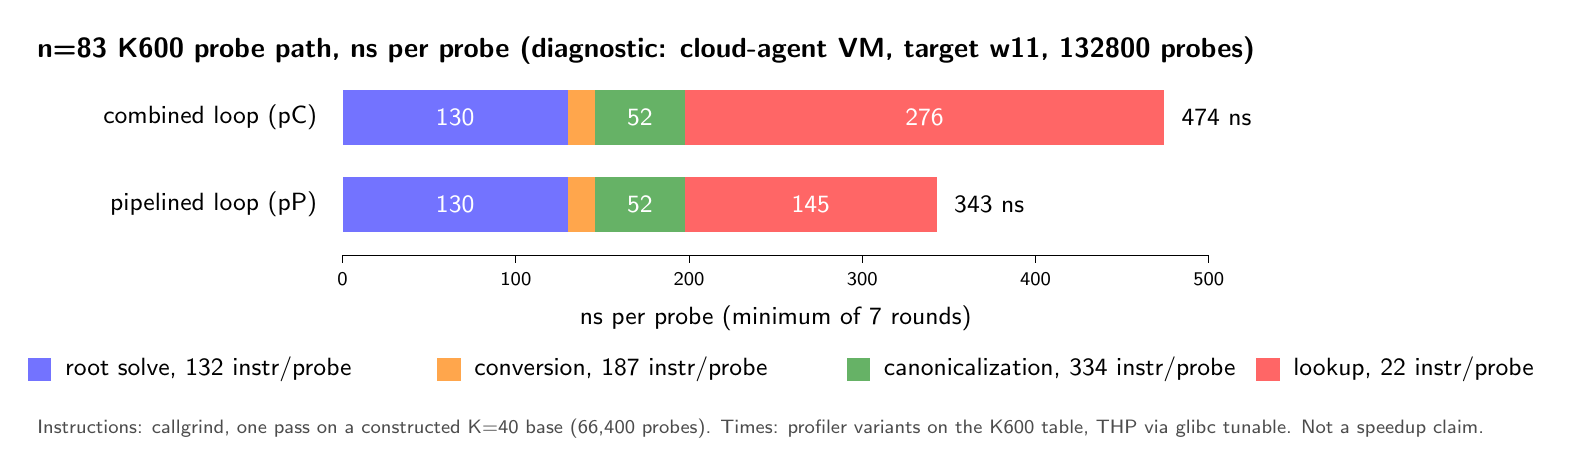
\begin{tikzpicture}[font=\sffamily\small]
\node[anchor=west,font=\sffamily\bfseries] at (0,3.2) {n=83 K600 probe path, ns per probe (diagnostic: cloud-agent VM, target w11, 132800 probes)};
\node[anchor=east] at (3.8,2.35) {combined loop (pC)};
\fill[blue!55] (4.000,2.00) rectangle (6.858,2.70);
\node[white] at (5.429,2.35) {130};
\fill[orange!70] (6.858,2.00) rectangle (7.200,2.70);
\fill[green!50!black!60] (7.200,2.00) rectangle (8.349,2.70);
\node[white] at (7.775,2.35) {52};
\fill[red!60] (8.349,2.00) rectangle (14.430,2.70);
\node[white] at (11.390,2.35) {276};
\node[anchor=west] at (14.530,2.35) {474 ns};
\node[anchor=east] at (3.8,1.25) {pipelined loop (pP)};
\fill[blue!55] (4.000,0.90) rectangle (6.858,1.60);
\node[white] at (5.429,1.25) {130};
\fill[orange!70] (6.858,0.90) rectangle (7.200,1.60);
\fill[green!50!black!60] (7.200,0.90) rectangle (8.349,1.60);
\node[white] at (7.775,1.25) {52};
\fill[red!60] (8.349,0.90) rectangle (11.543,1.60);
\node[white] at (9.946,1.25) {145};
\node[anchor=west] at (11.643,1.25) {343 ns};
\draw (4,0.6) -- (15.000,0.6);
\draw (4.000,0.6) -- (4.000,0.5) node[below,font=\sffamily\scriptsize] {0};
\draw (6.200,0.6) -- (6.200,0.5) node[below,font=\sffamily\scriptsize] {100};
\draw (8.400,0.6) -- (8.400,0.5) node[below,font=\sffamily\scriptsize] {200};
\draw (10.600,0.6) -- (10.600,0.5) node[below,font=\sffamily\scriptsize] {300};
\draw (12.800,0.6) -- (12.800,0.5) node[below,font=\sffamily\scriptsize] {400};
\draw (15.000,0.6) -- (15.000,0.5) node[below,font=\sffamily\scriptsize] {500};
\node at (9.500,-0.2) {ns per probe (minimum of 7 rounds)};
\fill[blue!55] (0.00,-1.0) rectangle ++(0.3,0.3);
\node[anchor=west] at (0.35,-0.85) {root solve, 132 instr/probe};
\fill[orange!70] (5.20,-1.0) rectangle ++(0.3,0.3);
\node[anchor=west] at (5.55,-0.85) {conversion, 187 instr/probe};
\fill[green!50!black!60] (10.40,-1.0) rectangle ++(0.3,0.3);
\node[anchor=west] at (10.75,-0.85) {canonicalization, 334 instr/probe};
\fill[red!60] (15.60,-1.0) rectangle ++(0.3,0.3);
\node[anchor=west] at (15.95,-0.85) {lookup, 22 instr/probe};
\node[anchor=west,font=\sffamily\scriptsize,text=black!70] at (0,-1.6) {Instructions: callgrind, one pass on a constructed K=40 base (66,400 probes). Times: profiler variants on the K600 table, THP via glibc tunable. Not a speedup claim.};
\end{tikzpicture}
\end{document}
